\documentclass[a4paper,12pt,twopage,swedish]{article}
\usepackage{amsmath,amssymb,mathrsfs}
\usepackage[utf8]{inputenc}
\usepackage{blindtext}
\usepackage{graphicx}
\usepackage[swedish]{babel}
\usepackage[margin={1in, 1in}]{geometry}
%\usepackage{mathtools}
\setlength{\parindent}{0pt}
\renewcommand{\thetable}{\Alph{table}}
%----------------------------------------------------------------------------
\begin{document}

%=================================================================
\title{Stelkroppssimulering}
%----------------------------------------------------------------------------
\author{Tomas Forsyth Rosin, Jonas Zeitler, Emil Axelsson, Karl Johan Krantz}
\begin{titlepage}
\maketitle
\thispagestyle{empty}
\end{titlepage}
%----------------------------------------------------------------------------
\setcounter{page}{1}
\pagenumbering{roman}
\begin{abstract}
Sammanfattning av projektet.
\end{abstract}
\clearpage
%----------------------------------------------------------------------------
\tableofcontents
\clearpage
%----------------------------------------------------------------------------
\listoffigures
\clearpage
%----------------------------------------------------------------------------
\listoftables
\clearpage
%----------------------------------------------------------------------------
\setcounter{page}{1}
\pagenumbering{arabic}

\section{Inledning}

\subsection{Bakgrund}
Fysiksimulering är en vital del av många moderna datorspel. I spelsammanhang kallas detta för ett spels \emph{fysikmotor}. Att implementera en fysikmotor handlar om att skapa en miljö med regler till vilka en uppsättning objekt måste förhålla sig. I många spel utgörs fysikmotorns bas av en \emph{stelkroppssimulering}, vilket innebär vissa antaganden och förenklingar av verkligheten. Mest påtagligt är att systemets objekt antas vara okomprimerbara, eller stela. Även med dessa förenklingar i beaktning är implementation av en fysikmotor ett komplext problem, som kan lösas på olika sätt beroende på aktuella förutsättningar och tillämpningsområden.

\subsection{Syfte}
Syftet med denna rapport är att beskriva utvecklingen av en fysikmotor, som ska kunna användas i datorspel med tvådimensionell grafik. Motorn ska ha stöd för att simulera kollisioner och friktion mellan stelkroppar modellerade som generella konvexa polygoner. Den ska också innehålla stöd för fjädrar och dämpare, som ska kunna fästas i stelkropparna. Motorn ska producera trovärdiga resultat vid såväl kollisioner som när flera stelkroppar vilar på varandra. Eftersom motorn ska kunna användas till datorspel behöver algoritmerna som används vara tillräckligt tidseffektiva för att tillåta interaktivitet. Motorn ska implementeras i C++ med hjälp av grafikbiblioteket OpenGL varpå resultatet ska utvärderas i rapporten.

%----------------------------------------------------------------------------

\section{Modell}
I modellen som skulle simuleras ingick tre typer av entiteter: rörliga stelkroppar, fasta stelkroppar samt fjädrar med dämpning. Varje entitet kan ha både konstanta egenskaper och variabla tillstånd, enligt tabell \ref{table:states_and_properties}.

\begin{table}[!htp]
	\caption{Tillstånd och egenskaper hos olika entiteter}
	\label{table:states_and_properties}
	\renewcommand{\arraystretch}{1.5}
	\begin{tabular}{|p{1cm}|p{1cm}|p{1cm}|p{1cm}|p{1cm}|p{1cm}|}
		\hline
			\multicolumn{2}{|c|}{\textbf{Rörliga stelkroppar}} & \multicolumn{2}{|c|}{\textbf{Fasta stelkroppar}} & \multicolumn{2}{|c|}{\textbf{Fjädrar med dämpare}} \\
		\hline
			\textbf{Tillstånd} & \textbf{Egenskaper} & \textbf{Tillstånd} & \textbf{Egenskaper} & \textbf{Tillstånd} & \textbf{Egenskaper} \\
		\hline
			Position & Densitet & & Position & & Infästnings\-punkter \\
			Vinkel & Studs\-koefficient & & Vinkel & & Fjäder\-konstant \\
			Hastighet & & & & & Dämpnings\-koefficient \\
			Vinkel\-hastighet & & & & & {} \\
		\hline
	\end{tabular}
\end{table}












\clearpage \clearpage
%------------------------------------------------------------------------------------








\section{Kollisionslösning}
	Att två objekt interpenetrerar varandra representerar inget verkligt fysikaliskt förlopp. Det första som därför måste göras när en sådan händelse upptäckts är att flytta ut objekten från varandra. En metod för detta är att hitta det tidssteg mellan innevarande och föregående bildruta då objekten kolliderade. En analytisk lösning är emellertid komplicerad att implementera med tanke på translations- och rotationshastigheter. En enklare metod är att hitta den punkt hos polygon A som interpenetrerar längst och betrakta den sida på polygon B som ligger närmast denna punkt som en trolig kollisionssida. Hur objekten sedan separeras från varandra går att lösa på olika sätt - linjärt 
	\subsection{Expanding Polytope Algorithm (EPA)}
		I denna tillämpning användes metoden EPA (Expanding Polytope Algorithm) för att hitta penetrationspunkten och en vektor mellan denna punkt och kollisionssidan, nedan kallad penetrationsvektorn. I det konvexa höljet av Minkowskidifferensen, beskriven i avsnitt \ref{sec:gjk}, kommer den linje med minst avstånd till origo att vara av intresse. De punkter som spänner upp denna linje har genererats utifrån penetrationspunkten, i  BEHÖVER FIGUR benämnd c, och de två punkter, d och e, som spänner upp kollisionssidan.
	\subsection{Linjär Kollisionslösning}
		\begin{figure}[!h]
			\centering
			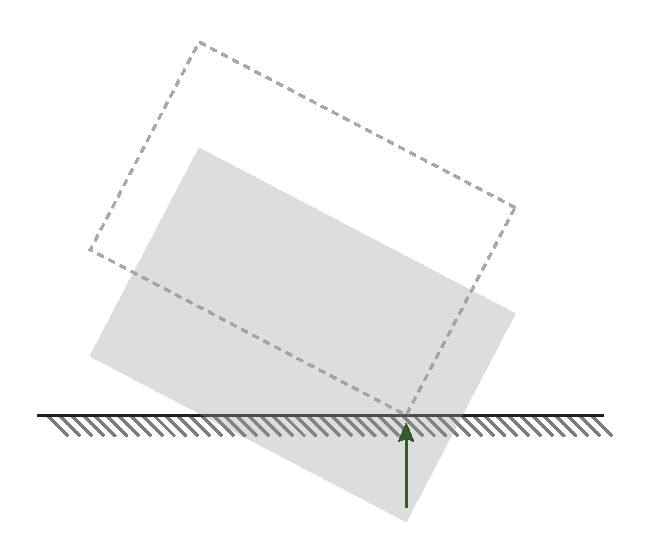
\includegraphics{illustrations/linear.pdf}
			\caption{Exempel på linjär utflyttning}
			\label{fig:linear}
		\end{figure}
		En linjär kollisionslösning är det enklaste sättet att lösa interpenetration. Penetrationen löses sådant att kropparna a och b (Figur \ref{fig:linear}) translateras i penetrationsvektorns positiva respektive negativa riktning. Hur stor del av penetrationsvektorn respektive kropp skall translateras beräknas med avseende på dess omvända relativa massa enligt (\ref{eq:impulse_part}).
		\begin{equation}\label{eq:impulse_part}
			J_{part} = \frac{m1}{m1+m2}
		\end{equation}
		Att translatera en rörlig kropp ut från en stationär kropp utan att påverka dess hastighet medför en förändring av systemets energi. För att motverka detta beräknas hastigheten om med avseende på utflyttningen och gravitationen.
		\begin{equation}\label{eq:v_magnitude}
			|\bar{v}| = \sqrt{|v^{2}-2\cdot|g_y| \cdot t_y|}
		\end{equation}
		Ekvation (\ref{eq:v_magnitude}) beskriver den nya hastigheten $v$ där $t$ är kroppens utflyttningsvektor och $g$ är den aktuella gravitationen för systemet.
	\subsection{Icke-linjär kollisionslösning}

		Linjära lösningar för interpenetration skapar problem för kroppar i vila. Detta eftersom gravitationen påverkar kropparna vilket resulterar i interpenetration med underlaget. Detta resulterar i sin tur i en linjär utflytt med avseende på den punkt med längst penetrationsvektor. För kroppar i vila innebär detta att de kommer vibrera istället för att ligga stilla. Dessutom kan det visas att oönskad friktion introduceras i systemet. Ett förslag till förbättring är att dela upp utflytt av en kropp till två komponenter. En linjär förflyttningskomponent med avseende på kroppens tröghet (\ref{eq:mass_mass_inertia_part}) och en rotationskomponent med avseende på kroppens tröghetsmoment (\ref{eq:inertia_mass_inertia_part}).
		
		\begin{equation}\label{eq:mass_mass_inertia_part}
		 	lm_i = \frac{\frac{1}{m_i}}{\frac{1}{m_1} + \frac{1}{m_2} + \frac{1}{I_1} + \frac{1}{I_2}}
		\end{equation}
		\begin{equation}\label{eq:inertia_mass_inertia_part}
		 	am_i = \frac{\frac{1}{m_i}}{\frac{1}{m_1} + \frac{1}{m_2} + \frac{1}{I_1} + \frac{1}{I_2}}
		\end{equation}

		I simuleringen implementerades endast den linjära utflyttningskomponenten (\ref{eq:mass_mass_inertia_part}) och sedan en explicit lösning (Figur \ref{fig:nonlinear}) för hur kroppen ska roteras ut.
				
						\begin{figure}[h!]
							\centering
							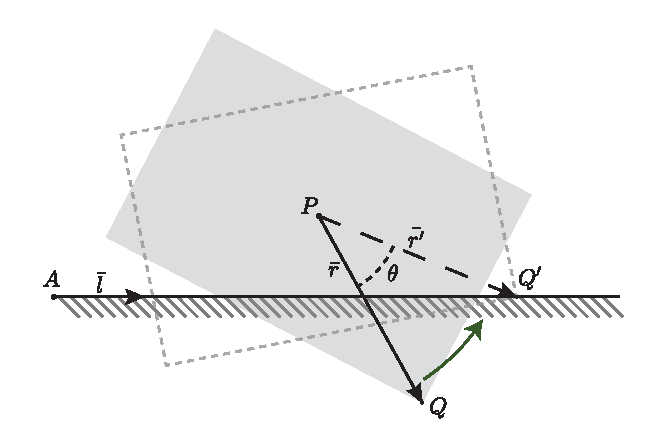
\includegraphics{illustrations/nonlinear.pdf}
							\caption{Exempel på icke-linjär utflyttning}
							\label{fig:nonlinear}
						\end{figure}
		
		Metoden innebär att lösa ett ekvationssystem med fyra rötter och sedan testa vilken lösning som ger den optimala, dvs. minsta,  rotationen ut.
		\begin{equation} \label{eq:nonlinear_1}
			Q' = P + \bar{r}' = A + s \cdot \bar{l}
		\end{equation}
		\begin{equation}\label{eq:nonlinear_2}
			|\bar{r}|^2 = |\bar{r}'|^2 = (Q-P)^2 = (Q' - P)^2
		\end{equation}
		\begin{equation}\label{eq:nonlinear_3}
			\theta = \arccos{\frac{\bar{r}\cdot\bar{r} '}{|\bar{r}|^2}}
		\end{equation}
		Från (\ref{eq:nonlinear_1}) och (\ref{eq:nonlinear_2}) löses $\bar{r}'$ut och rotationen beräknas enligt (\ref{eq:nonlinear_3}).

		För djupa penetrationer mellan kroppar med stor tröghet kan den linjära komponenten inte räcka för att lösa interpenetrationen utan gör att rotationen förvärrar interpenetrationen. I dessa fall kan en nedre gräns för den linjära komponenten införas för att vikta förhållandet mellan rotation och translation [BEHÖVER REFERENS].




%----------------------------------------------------------------------------
\section{Kollisionsdetektion}

Det första steget mot att simulera stelkroppars interaktion är att detektera alla kolliderande polygoner i scenen. Att två objekt i ett diskret system ligger dikt an varandra är sällsynt. Vanligare är att de interpenetrerar varandra, d.v.s. att ett hörn hos ett objekt ligger inuti ett annat objekt.

\subsection{Detektionsmetod}

I detta projekt diskuterades i huvudsak två metoder för kollisionsdetektion.

\subsubsection{Separating Axis Test}
För att utreda eventuell interpenetration mellan två givna objekt kan SAT \cite[s.~29]{vella08} \emph{(Separating Axis Test)} användas. Testet kan avgöra om objekten inte kolliderar genom att hitta en vektor på vilken objektens punkter projiceras på disjunkta intervall (Figur ~\ref{fig:disjoint_intervals}). Ett högre antal vektorer ökar beräkningstiden men också sannolikheten för ett korrekt resultat.

\subsubsection{Gilbert-Johnson-Keerthi}
För att inte göra avkall på noggrannheten har en annan metod, GJK \cite[s.~30]{vella08} \emph{(Gilbert-Johnson-Keerthi)}, använts för detta projekt. Eftersom metoden kan utesluta fler möjliga kollisioner kommer senare beräkningar kräva mindre tid. GJK bygger på Minkovskidifferensen mellan de två objekten, definierad enligt (\ref{eq:minkovski_difference}).

\begin{equation}\label{eq:minkovski_difference}
\chi_1 \ominus \chi_2 = \{x_1 - x_2|x_1 \in \chi_1, x_2 \in \chi_2\}
\end{equation}

De två objekten korsar varandra om, och endast om, polygonen som Minkovskidifferensen renderar innehåller origo. GJK-algoritmen utreder detta på ett sätt som minskar antalet beräkningar från polynomiellt till linjärt beroende av antalet punkter i objekten \cite{bergen99}.

\subsection{Optimering}

Att undersöka kollisioner för alla par av objekt i varje bildruta medför omfattande beräkningar och sänker programmets effektivitet betydligt. För att undvika dessa beräkningsmängder görs först olika bedömningar av vilka objekt som riskerar att kollidera varefter de tyngre kollisionsdetektorerna appliceras endast på dessa par.

\subsubsection{Bounding boxes}

För att förenkla representationen av objekt användes Bounding Boxes. För varje punkt i objektet beräknas den maximala respektive minimala koordinaten i alla dimensioner. Av dessa värden konstrueras sedan nya punkter som bildar ett rätblock (rektangel i två dimensioner) med sidor parallella med koordinataxlarna. Alla punkter i objektet kommer att ligga i detta rätblock vilket gör att man snabbt kan utesluta förekomster av punkter i stora områden.

\subsubsection{Quadtree}


%----------------------------------------------------------------------------
\section{Kollisionslösning}
%----------------------------------------------------------------------------
\section{Kollisionsrespons}
%----------------------------------------------------------------------------
\section{Krafter i impuls-\\baserade system}

\subsection{Kraftgeneratorer}

Hittills har endast impulser mellan objekt diskuterats. Impulser är emellertid en förenkling av vad som egentligen sker i stötar och kontakt. En kollision mellan två objekt orsakar kompression hos materialen i respektive objekt vilket i sin tur ger upphov till statiska, motriktade, krafter (kraft/motkraft enligt Newton 3 \cite{newton87}). Dessa krafter verkar inte momentant utan under ett tidsspann. Impulser, som antas vara momentana, kan därför relateras till krafter enligt  (\ref{eq:impulse_force_relation}).

\begin{equation}\label{eq:impulse_force_relation}
J = \int\limits_{\Delta t} F \,dt\
\end{equation}

Vissa fysikmotorer delar upp tiden i varje tidssteg i mindre delar och kan på så sätt erhålla en bättre approximation för vissa krafter. Dessa metoder kallas tidsderiverande. ...

\subsection{Friktion}

Den allra vanligaste friktionsmodellen är Coloumbs modell. Den baserar sig i att den friktionskraften som påverkar ett objekt är proportionell mot normalkraften mellan objektet och underlaget. Modellen är egentligen en sammanslagning av två modeller, statisk och dynamisk friktion. Där den statiska modellen används för objekt i vila och den dynamiska för objekt i rörelse.

\begin{equation}\label{eq:static_friction}
f_d = \mu_d \cdot N
\end{equation}

\begin{equation}\label{eq:dynamic_friction}
f_s = \mu_s \cdot N
\end{equation}

\subsection{Fjäderkrafter}
%----------------------------------------------------------------------------
\section{Resultat}
%----------------------------------------------------------------------------
\section{Diskussion}
\clearpage
%=================================================================
\begin{thebibliography}{9}

\bibitem{vella08}
  Vella Colin,
  \emph{Gravitas: An extensible physics engine framework using object-oriented and design pattern-driven software architecture principles}.
  2008.

\bibitem{millington07}
  Millington Ian,
  \emph{Game Physics Engine Development}.
  2007.

\bibitem{bergen99}
  Van den Bergen Gino,
  \emph{A Fast and Robust GJK Implementation for Collision Detection of Convex Objects, Journal of Graphics Tool}.
  4:2, 7-25,
  1999.

\bibitem{newton87}
  Newton, Isaac
  \emph{Philosophiæ Naturalis Principia Mathematica}.
  1687.

\end{thebibliography}
\end{document} 